%\begin{figure}
%\centering
%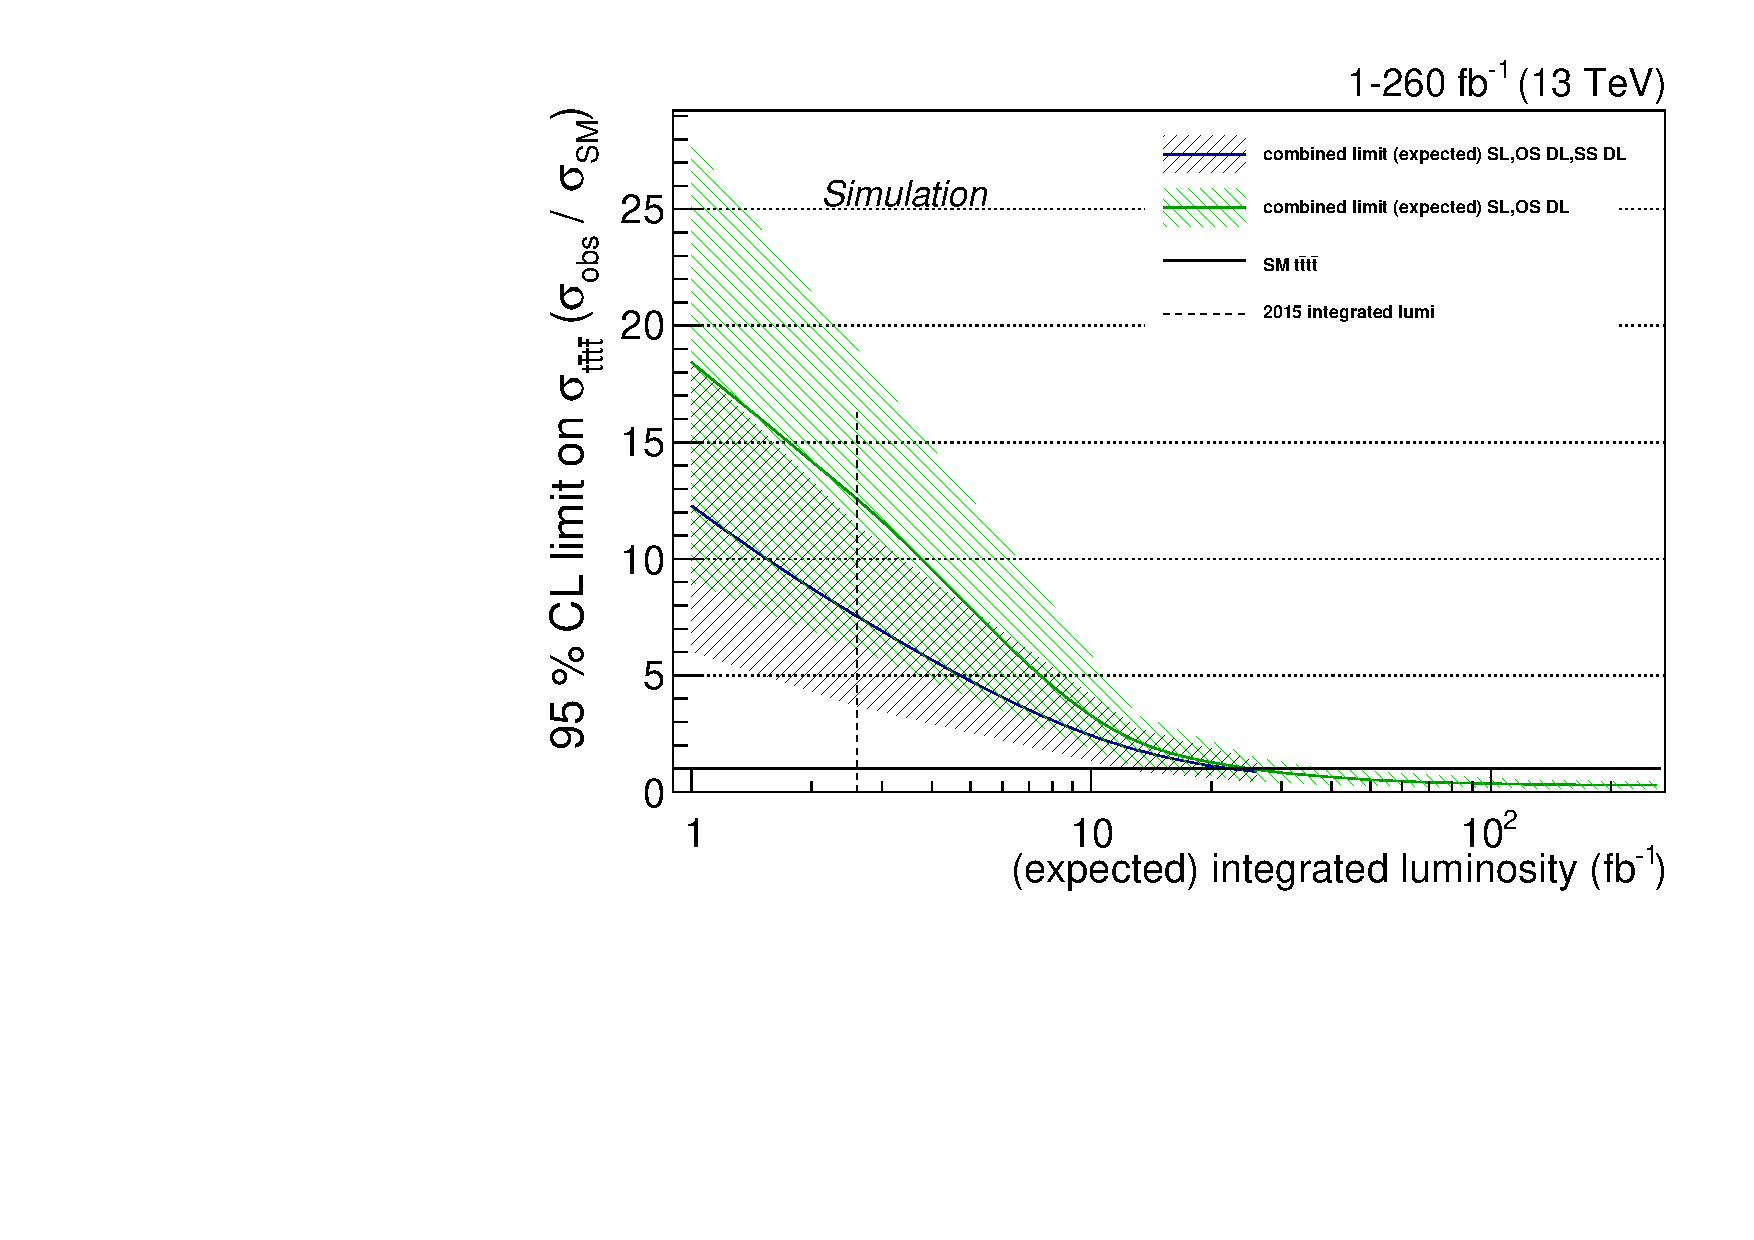
\includegraphics[width=0.45\linewidth]{./figures/combined_limitvslumi_fwo}
%\caption{Extrapolation, based on 2015 results~\cite{CMS:2016wig}, of the expected limit on the SM four top quark production cross section as a function of integrated luminosity of the dataset. Solid lines and hatched areas show expected limit dependence and one standard deviation uncertainty band, respectively, for single-lepton (SL) and opposite-sign di-lepton (OS DL) SM $t\bar{t}t\bar{t}$ search (blue) and single-lepton and same (SS DL) and opposite-sign dilepton search (green). The predictions performed assuming that the experimental uncertainty is dominated by statistical component. Even in the case of downward statistical fluctuation, the dataset  delivered during the time covered by this proposal (120 fb$^{-1}$) will be sufficient to observe this process.}
%\label{fig:combined_limitvslumi}
%\end{figure}
\textcolor{\mycolor}{
With this project \textbf{I plan to perform direct search for BSM processes in events with $\pmb{t\bar{t}t\bar{t}}$ signature  as well as measure four top quark production in $pp$ collisions with the CMS detector at the LHC at centre-of-mass energy $\sqrt{s}=$ 13 and 14 TeV.} The SM measurement aims at testing the state-of-the-art perturbative QFT predictions~\cite{Bevilacqua:2012em,Frederix:2017wme} while direct searches seek for BSM signal. As described above, there is a certain class of models predicting significantly larger than SM cross section values and resonances~\cite{Lillie:2007hd, Gregoire:2011ka, Pomarol:2008bh}, thus making direct test of such models at the LHC feasible in the RUN 2 for which, in total, more than 150 fb$^{-1}$ of the integrated luminosity are expected. The discovery of significant deviation from the SM predictions may have a major impact on the field, while the converse will help to restrict possible BSM scenarios. The recently published constraints from $\sqrt{s}=13$ TeV data for SM four top production at ATLAS~\cite{Aaboud:2017faq} and CMS~\cite{Sirunyan:2017tep}, to one of which I have made a leading contribution,
%~\cite{Aad:2015kqa,Khachatryan:2014sca} 
resulted in 60 and 69 fb 95\% CL upper limits on the production cross section, respectively. The study~\cite{Sirunyan:2017roi} reported the first observation of $t\bar{t}t\bar{t}$ production in multilepton channel. In this study small excess, although consistent with SM predictions, was observed. However, the measurement features about 80\% uncertainty on the measured cross section and is still dominated by statistical component.
}
\textcolor{\mycolor}{
The previous analysis at CMS in single-lepton and opposite sign dilepton channels made use of 2.3 fb$^{-1}$ of integrated luminosity, that is about 20 signal events for the complete 2015 dataset. \textbf{I plan to analyse full data sample collected in 2016--2018 to improve statistical and systematic accuracy of the search}. These datasets will significantly increase the sensitivity to the processes with four top quarks.}

\begin{figure}[t!]
\centering
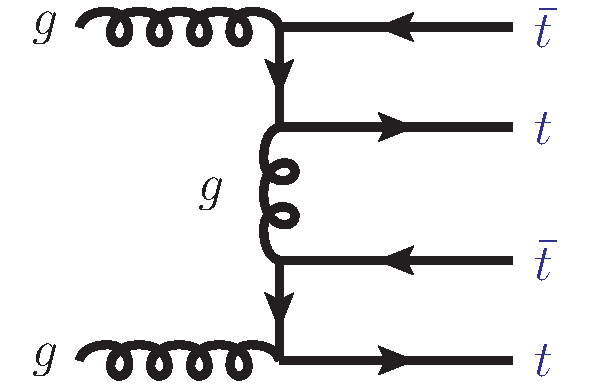
\includegraphics[width=0.25\textwidth]{Feynman/gg2tttt}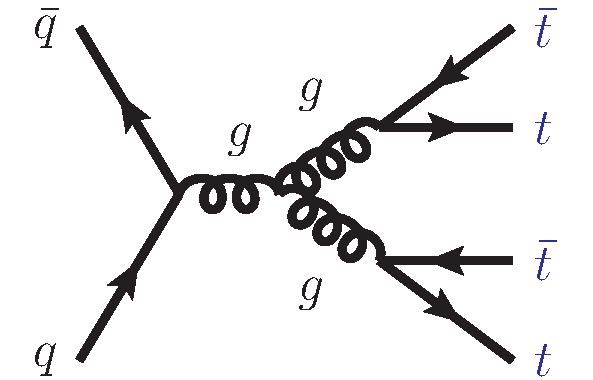
\includegraphics[width=0.25\textwidth]{Feynman/qq2tttt}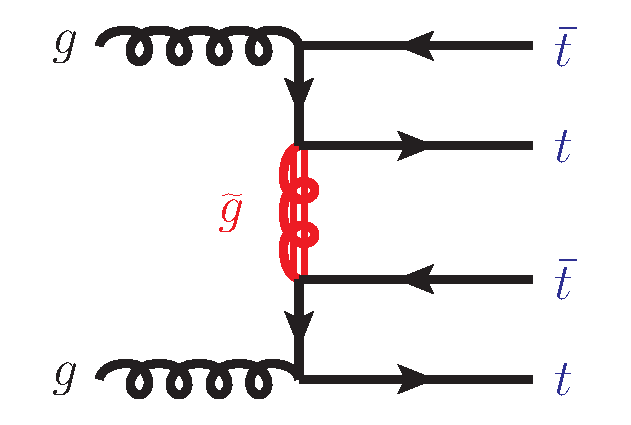
\includegraphics[width=0.25\textwidth]{Feynman/gg2ttttsgluon}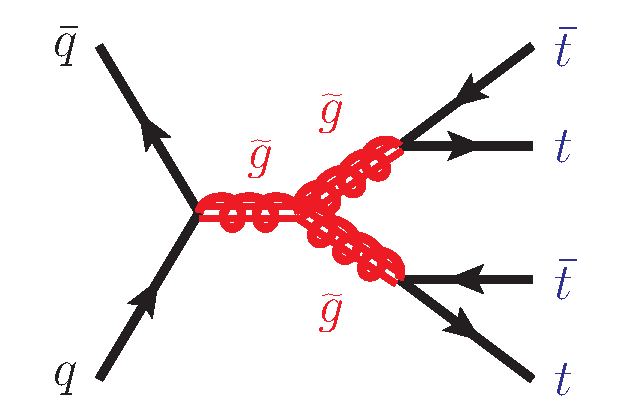
\includegraphics[width=0.25\textwidth]{Feynman/qq2ttttsgluon}
\caption{Examples of leading order SM and corresponding BSM Feynman diagrams for $t\bar{t}t\bar{t}$ production. The intermediate states, indicated by $\tilde{g}$, represent coloured scalar fields -- sgluons.}
\label{fig:LOtttt}
\end{figure}

\textcolor{\mycolor}{
Examples of leading order (LO) SM and corresponding BSM Feynman diagrams for $t\bar{t}t\bar{t}$ production are illustrated in Figure~\ref{fig:LOtttt}. The reconstruction of this process is especially challenging because such final state is characterised by large hadronic activity, $\hight$, and incorporates four b-quarks, jets or leptons from $W$-decays and additional jets from initial and/or final-state QCD radiation. In addition, such events have non-vanishing missing momentum in case of semileptonic $W$-decays, which is reasonably well under control in top physics. Bottom quarks are identified exploiting the properties of the weak decays of $B$-hadrons, which are typically formed from $b$'s during the hadronisation stage. These hadrons have relatively long mean lifetime of the order of 10$^{-12}$s and travel several millimeters from the production point before they decay giving rise to displaced tracks. Depending on the decay channel of $W$-bosons, several possible combinations of jet and lepton multiplicities can be identified in \fourtop events e.g. final states with a single muon $\left(\mu\right)$+jets or a single electron $\left(e\right)$+jets\footnote{In the following, charged first and second generation leptons, i.e. $e/\mu$ are generically denoted by $l$.} arising promptly from $W$ decays or in a cascade $W\rightarrow\tau\nu_\tau$, $\tau\rightarrow l\nu_l \nu_\tau$. This final state has the highest probability ($\approx 41\%$) of occurrence, while zero-leptons, two-leptons or three- and four-leptons have 30\%, 22\% and 6\% odds, respectively~\cite{Khachatryan:2014sca}. Vanishing $\misspt$ in the all-hadronic channel as well as the capability to reconstruct the momentum of the neutrino\footnote{The SM decay hypothesis of the $W$ boson has to be assumed} in the single-lepton channel, increases the sensitivity to BSM models without undetectable particles carrying significant momentum. This signature makes this proposal \textbf{unique as no similar analyses, besides ongoing effort of the applicant and the hosting group, are currently being performed by the CMS collaboration}.}

\textcolor{\mycolor}{
Several principal challenges inherent to the explored final state can be identified early on. 
%An efficient $b$-tagging algorithm with high discriminating power at high jet multiplicity is crucial for selection of four top events and suppression of overwhelming background, mostly comprised of $t\bar{t}jj$ production, where $jj$ denotes a pair of light-flavour\footnote{Jets originating from $u,d,s,g$ partons are generically called light-flavour jets.} or $c$-quark jets, or associated electroweak-boson production. The CMS collaboration relies on well established algorithms~\cite{Chatrchyan:2012jua} for this task. However, their settings were optimised for the physics environment of $\sqrt{s}=7(8)$ TeV runs~\cite{CMS:2013vea}, whereas due to increased energy and pile-up in RUN2, their performance may not be optimal anymore. Besides the pile-up effect, $b$-tagging may also be affected by the complex multijet signature of the proposed signal. Thus, \textbf{investigation and optimisation of $b$-tagging performance} in the complex $t\bar{t}t\bar{t}$ environment at $\sqrt{s}=$ 13(14) TeV is envisaged in this project. These results can be later used in other analyses with similar event signatures. 
A difficulty persistent to the reconstruction of multiple top quarks is identification of a correct combination of final state objects arising from a common mother-particle decay. For example, in the single-lepton channel, $4!\cdot C_6^2 \cdot C_4^2 = 2160$, where $C_n^k$ denotes binomial coefficient, possible assignments of four $b$-jets and six light-flavour jets to four top quarks exist. In order to suppress combinatorial background, decay products kinematic information can be used, e.g. combinations with invariant masses outside $W$-boson and top-quark mass windows can be rejected. Furthermore, MVA techniques can be applied to enhance classification power of assignment algorithm. The \textbf{improvement in the top-decay reconstruction} will have a significant impact on the signal sensitivity and background suppression.}

\textcolor{\mycolor}{
The details of the suggested solutions to foreseen challenges as well as the generic strategy for reaching the objectives of this proposal are outlined below.}
%The principal goal and major challenges can be 
% 
%\textbf{TODO:}\\
%- Describe how to search for four top events. Many jets, many b's,\\
%\hfill
%+ Test of the SM predictions and search for BSM signatures.\\
%+ So far 32fb-1 limit was established while SM cross section is only 1fb-1 and this gives a huge room where to hide for new physics.\\
%+ It is very important and will have a huge impact in case of discovery and will place strict limits on possible BSM scenarios.\\
%+ It is very challenging because of overwhelming SM background, possibly not enough efficient b-tagging etc.;
%+++ enumerate probabilities for four top decay channels+++
%+++Mention b-classification efficiency+++ 
%+++Mention combinatorics problem+++ 
%+++Mention QCD background+++ 
%+++Mention non-optimal b-tagging for increased pile-up/boosted jets (timely)+++
%+++Mention possibly non-optimal trigger+++